\section{Case study: weight decay improves robustness to data repetition}
\label{sec:results}

The overfitting coefficient directly quantifies a training configuration's robustness to data repetition. To demonstrate this, we analyze the effect of weight decay strength on repetition tolerance, training the same grid of model sizes and data budgets at two settings: standard $\lambda = 0.1$ and strong $\lambda = 1.0$ weight decay, with all other hyperparameters held constant.

\begin{figure}[t]
    \centering
    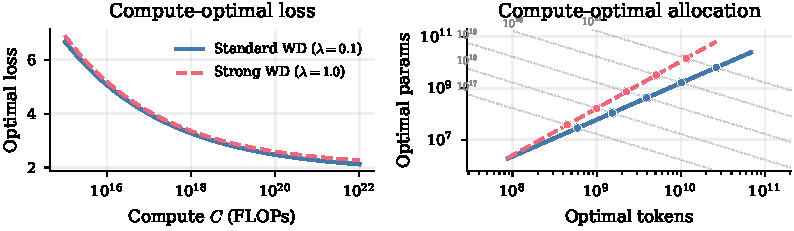
\includegraphics[width=\textwidth]{figures/wd_chinchilla_optimal.pdf}
    \caption{\textbf{Strong weight decay incurs a single-epoch loss premium.} \textbf{(Left)}~Compute-optimal frontier: strong weight decay ($\lambda=1.0$) achieves higher loss than the standard setting at every compute budget in the single-epoch regime. \textbf{(Right)}~Compute-optimal allocation: strong weight decay favors larger models relative to data.}
    \label{fig:single_epoch_wd}
    \vspace{-.5em}
\end{figure}

\para{Single-epoch scaling.} We fit separate Chinchilla parameters $(A, B, E, \alpha, \beta)$ per setting. In the single-epoch regime, strong weight decay incurs a loss premium at every compute budget (\autoref{fig:single_epoch_wd}), and its compute-optimal allocation favors larger models relative to data.

\begin{figure}[t]
    \centering
    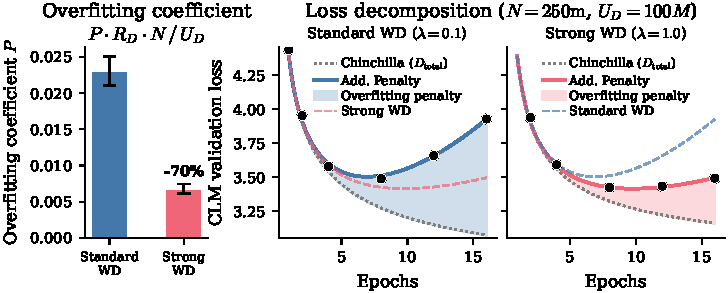
\includegraphics[width=\textwidth]{figures/wd_decomposition_data_250m_100M.pdf}
    \caption{\textbf{Strong weight decay improves robustness to data repetition.} \textbf{(Left)}~Fitted overfitting coefficient $P$ for standard ($\lambda=0.1$) and strong ($\lambda=1.0$) weight decay; strong weight decay reduces $P$ by approximately 70\%. \textbf{(Center, Right)}~Loss decomposition for a 250M-parameter model trained on 100M unique tokens across weight decay values.}
    \label{fig:loss_decomposition}
    \vspace{-1em}
\end{figure}

\para{Scaling under data repetition.} We fit our additive penalty (\autoref{eq:four_param}) independently for both weight decay settings.
\autoref{fig:loss_decomposition} (left) shows the fitted $P$ values from the one-parameter form (\autoref{eq:one_param}): strong weight decay reduces $P$ by approximately 70\%, meaning it incurs far less overfitting per repetition. The loss decomposition for a representative configuration (center, right) shows the overfitting penalty growing superlinearly for both settings, but with significantly lower magnitude under strong weight decay.

\para{Crossover under repetition.} Although there is a single-epoch loss premium, the significantly reduced overfitting cost creates a crossover point in performance (\autoref{fig:crossover_multi}). At $U_D = 250$M, standard weight decay achieves lower loss at modest compute, but strong weight decay overtakes it at $C \approx 3.2 \times 10^{18}$ FLOPs as the standard setting's steeper penalty erodes its single-epoch advantage. Our scaling law predicts this crossover point: the compute budget at which the lower penalty compensates for the single-epoch tax.

\begin{figure}[t]
    \centering
    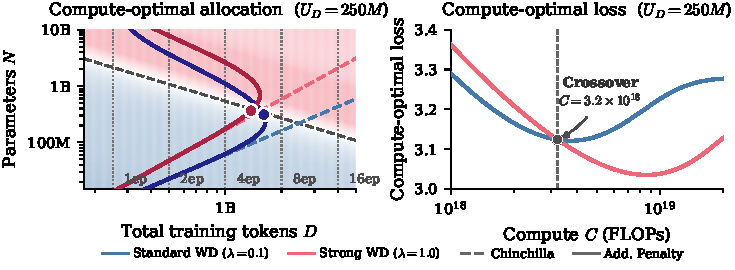
\includegraphics[width=\textwidth]{figures/allocation_comparison_250M.pdf}
    \caption{\textbf{Strong weight decay outperforms in high-compute regimes.} \textbf{(Left)}~Compute-optimal allocation frontiers for standard ($\lambda=0.1$) and strong ($\lambda=1.0$) weight decay at $U_D = 250$M. \textbf{(Right)}~Compute-optimal loss as a function of compute budget. Strong weight decay incurs higher loss at low compute but crosses over at $C \approx 3.2 \times 10^{18}$ FLOPs.}
    \label{fig:crossover_multi}
    \vspace{-1em}
\end{figure}

\begin{table}[t]
    \centering
    \caption{\textbf{Weight decay prescriptive validation.} For each (token budget, compute budget) pair, we train the configuration recommended by our scaling law (\autoref{eq:four_param}). Standard weight decay ($\lambda = 0.1$) achieves lower loss at small compute budgets, but strong weight decay ($\lambda = 1.0$) enables productive use of additional compute, ultimately achieving lower absolute loss. We denote the expected crossover point under our law with $C^{\times}$.}
    \label{tab:wd_validation}
    \begin{tabular}{llllrrr}
        \toprule
        $U_D$ & $C$ & Weight Decay & Params & Epochs & Perplexity $\downarrow$ & BPB  $\downarrow$\\
        \midrule
        \multirow{6}{*}{\makecell[l]{250M\\[0pt]{\small $C^{\times}\! \approx 3\!\times\!10^{18}$}}}
        & \multirow{2}{*}{\textcolor{gray}{$3 \times 10^{18}$}}
        & \textcolor{gray}{$\lambda = 0.1$} & \textcolor{gray}{350M} & \textcolor{gray}{6} & \textcolor{gray}{23.38} & \textcolor{gray}{1.46} \\
        & & \textcolor{gray}{$\lambda = 1.0$} & \textcolor{gray}{350M} & \textcolor{gray}{6} & \textcolor{gray}{22.93} & \textcolor{gray}{1.47} \\
        \cmidrule(l){2-7}
        & \multirow{2}{*}{$5 \times 10^{18}$}
        & $\lambda = 0.1$ & 700M & 5 & 22.91 & 1.47 \\
        & & $\lambda = 1.0$ & 550M & 6 & {21.66} & {1.41} \\
        \cmidrule(l){2-7}
        & \multirow{2}{*}{$1 \times 10^{19}$}
        & $\lambda = 0.1$ & 3B & 2 & 23.13 & 1.52 \\
        & & $\lambda = 1.0$ & 1B & 6 & {20.34} & {1.36} \\
        \midrule
        \multirow{4}{*}{\makecell[l]{500M\\[0pt]{\small $C^{\times}\!\approx 1\!\times\!10^{19}$}}}
        & \multirow{2}{*}{\textcolor{gray}{$1 \times 10^{19}$}}
        & \textcolor{gray}{$\lambda = 0.1$} & \textcolor{gray}{700M} & \textcolor{gray}{5} & \textcolor{gray}{18.52} & \textcolor{gray}{1.36} \\
        & & \textcolor{gray}{$\lambda = 1.0$} & \textcolor{gray}{830M} & \textcolor{gray}{4} & \textcolor{gray}{18.75} & \textcolor{gray}{1.32} \\
        \cmidrule(l){2-7}
        & \multirow{2}{*}{$3 \times 10^{19}$}
        & $\lambda = 0.1$ & 5B & 2 & 18.16 & 1.35 \\
        & & $\lambda = 1.0$ & 2.5B & 4 & {16.65} & {1.30} \\
        \bottomrule
    \end{tabular}
    \vspace{-1.5em}
\end{table}

\para{Prescriptive validation.} We validate on held-out configurations (\autoref{tab:wd_validation}). The results confirm the crossover dynamics predicted by our law. Near the predicted crossover budget $C^{\times}$, the two settings perform comparably. Beyond this point, the gap widens rapidly---at $C = 1 \times 10^{19}$ (${\sim}3\times$ past the crossover), strong weight decay reduces perplexity by 2.8 points. The same pattern holds at $U_D = 500$M: near the crossover the settings are comparable, but at $3 \times 10^{19}$ strong weight decay achieves 16.65 vs.\ 18.16 perplexity. Our law correctly predicts that strong weight decay should train for more epochs, and the recommended configurations achieve lower loss when the data constraint is binding. This provides prescriptive support for the empirical finding of \citet{kim2026pretraining} that optimal weight decay in data-constrained regimes can be an order of magnitude larger than standard practice. 